\mysection{Hierarchical Attention}

\vspace{1\baselineskip}


    \begin{minipage}[c]{0.3\textwidth}
        \centering
        \begin{subfigure}[b]{1.\textwidth}
            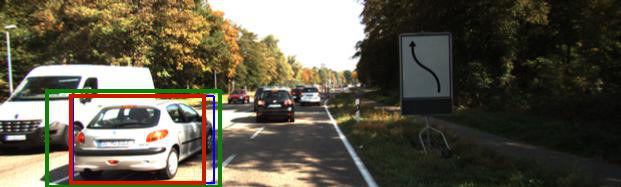
\includegraphics[width=\textwidth]{att_img}
%            \caption*{\textcolor{red}{prediction}, \textcolor{blue}{ground-truth}}
        \end{subfigure}
        
        \hspace{-30pt}
        \begin{minipage}{.9\textwidth}
            \centering
            \vspace{.5em}
            \begin{subfigure}[b]{.31\textwidth}
                \centering
                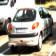
\includegraphics[width=\textwidth, cfbox=darkgreen 9pt 0pt]{att_glimpse}
                \caption*{\large attention glimpse}
            \end{subfigure}
            \hfill
            \begin{subfigure}[b]{.31\textwidth}
                \centering
                
\includegraphics[width=\textwidth, cfbox=white 9pt 0pt]{att_mask}
                \caption*{\large object mask}
            \end{subfigure}
            \hfill
            \begin{subfigure}[b]{.31\textwidth}
                \centering
                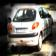
\includegraphics[width=\textwidth, cfbox=white 9pt 0pt]{att_overlay}
                \caption*{\large appearance attention}
            \end{subfigure}
            
        \end{minipage}
    \end{minipage}\hfill
    \begin{minipage}[c]{0.3\textwidth}
        \vspace{1\baselineskip}
        \begin{description}[labelsep=1em, leftmargin=!,labelwidth=\widthof{\bfseries Interpretable:}, itemsep=0.5em]
            \item[Bio-inspired:] Two-stream processing pathway and attention mechanisms adapted from human visual cortex.
            \item[Interpretable:] Important features selected by Spatial Attention and Object Segmentation mechanisms.
            \item[Scalable:] Applicable to real-world data due to\\ distractor suppression and auxiliary loss terms.
            \item[Efficient:] Attention quickly discards irrelevant features\\
                              $> 120$ fps on a laptop! 
        \end{description}
    \end{minipage}

%    \item[Why:] Attention Mechanisms adapted from Human Visual Cortex suppress distractors and increase efficiency 
%\item[Result:] Interpretable Neural Tracker applicable to Real-World Data 